\documentclass[../../FisicaTeorica.tex]{subfiles}

\begin{document}
%\section{?}
\subsection{Calcolo di probabilità}
%\lesson{15}{26/10/2018}
Dato un'osservabile $A$ e uno stato $\psi$, sia $P^A_\psi(\lambda)$ la famiglia spettrale di $A$, allora la probabilità di ottenere un risultato in un insieme $\Delta\subseteq \bb{R}$ misurando $A$ nello stato $\psi$ è data dalla formula generale:
\begin{equation}
P^A_\psi(\Delta) = \int_\bb{R} \chi_\Delta(\lambda)\,dP^A(\lambda)
\label{eqn:prob_generale}
\end{equation}
\subsubsection{Spettro discreto}
Se lo spettro dell'operatore è unicamente discreto, espandendo la (\ref{eqn:dPA_op}):
\[
dP^A_\psi(\lambda)\big|_{\sigma_P(A)}=\sum_{\lambda_n\in\sigma_P(A)}\delta(\lambda-\lambda_n)\sum_{r=1}^{d(\lambda_n)}\braket{\psi|\lambda_{n},r}\braket{\lambda_{n,}r|\psi}d\lambda
\]
dove gli autovettori generalizzati sono ortonormali:
\[
\braket{\lambda_{n},r|\lambda_{m},r'}=\delta_{nm}\delta_{rr'}
\]
Sostituendo tale risultato in (\ref{eqn:prob_generale}) si ottiene:
\begin{align}
P_\psi^A(\{\lambda_n\})&=\int_\bb{R} \chi_{\{\lambda_n\}}(\lambda)dP_\psi^A(\lambda)=\nonumber \\
&=
\int_\bb{R} d\lambda \chi_{\{\lambda_n\}}\sum_{\lambda_n\in\sigma_P(A)}\delta(\lambda-\lambda_m)\sum_{r=1}^{d(\lambda_m)}\braket{\psi|\lambda_{m},r}\braket{\lambda_{m},r|\psi} =\nonumber \\
&\underset{(a)}{=} \sum_{r=1}^{d(\lambda_n)}|\braket{\psi|\lambda_{n},r}|^2 = W^A_\psi(\lambda_n)
\label{eqn:probability_discreta}
\end{align}
Dove in (a) si è usata la definizione della funzione caratteristica:
\[
\chi_{\{\lambda_n\}}(\lambda)=
\begin{cases}
1 & \lambda=\lambda_n\\
0 & \text{altrove}
\end{cases}
\]
per far \q{collassare} l'integrale.\\
$P_\psi^A(\{\lambda_n\})$ è dunque la probabilità che una misura di $A$ nello stato $\psi$ restituisca $\lambda_n$.\\
\subsubsection{Spettro continuo}
Se lo spettro è continuo, la misura \q{non pesa i punti} (ossia i punti sono considerati insiemi Lebesgue-trascurabili) e quindi la probabilità di ottenere un certo (singolo) valore di $A$ è nulla. L'unica cosa che possiamo fare è definire una densità di probabilità:
\begin{equation}
w_\psi^A(\lambda)=\frac{dP_\psi^A(\lambda)}{d\lambda} = \sum_{r=1}^{d(\lambda)}|\langle\psi|\lambda,r\rangle|^2
\label{eqn:probability_continua}
\end{equation}
dato che:
\[
dP_\psi^A(\lambda)\Big|_{\sigma_C(A)}=\sum_{r=1}^{d(\lambda)}\braket{\psi|\lambda,r}\braket{\lambda,r|\psi}d\lambda
\]
Stiamo qui considerando i $\lambda$ normalizzati in modo che $\braket{\lambda,r|\lambda,r'}=\delta(\lambda-\lambda')\delta_{rr'}$.

\subsubsection{Applicazione alla buca infinita}
Applichiamo quanto appena trovato al caso della buca infinitamente profonda in una dimensione. In (\ref{eqn:evoluzione_buca_t}) avevamo ricavato l'evoluzione temporale del sistema a partire da uno stato iniziale, ottenendo:
\begin{equation}
\ket{\psi(t)}=\frac{1}{\sqrt{5}}\left(\exp\left(-i\frac{\mathcal{E}_1}{\hbar}(t-t_0)\right)\ket{\varphi_1}
+ 2\exp \left(-\frac{i}{\hbar}\mathcal{E}_2(t-t_0)\right)\ket{\varphi_2}
 \right)
 \label{eqn:evoluzione_buca_2}
\end{equation}
dove $\ket{\varphi_1}$ e $\ket{\varphi_2}$ sono autofunzioni dell'operatore hamiltoniana.\\
Proviamo allora a calcolare la probabilità di trovare $\mathcal{E}_1$ misurando $H$ in $\psi(t)$.\\
Abbiamo mostrato che lo spettro dell'hamiltoniana nel caso della buca infinitamente profonda tra $[-\frac{a}{2},\frac{a}{2}]$ è puramente discreto:
\[
\sigma(H)=\sigma_P(H)=\{\mathcal{E}_n = \frac{\hbar^2}{2m}\left(\frac{n\pi}{a} \right)^2,\>n\in\bb{N}\}
\]
Applicando allora la formula (\ref{eqn:probability_discreta}) otteniamo:
\begin{equation}
W_{\psi(t)}^H(\mathcal{E}_1) = |\braket{\psi(t)|\varphi_1}|^2
\label{eqn:calcolo_prob}
\end{equation}
dove $\ket{\varphi_1}$ è l'autofunzione di $H$ di autovalore $\mathcal{E}_1$, ossia verifica, in notazione di Dirac:
\[
H\ket{\varphi_1}=\mathcal{E}_1 \ket{\varphi_1}\Rightarrow \quad \ket{\varphi_1} = \ket{\mathcal{E}_1}
\]
Sostituendo allora (\ref{eqn:evoluzione_buca_2}) in (\ref{eqn:calcolo_prob}) e svolgendo i conti:
\begin{align*}
W_{\psi(t)}^H(\mathcal{E}_1) &= \left| \bra{\varphi_1}
\left (
\frac{1}{\sqrt{5}}\exp\left(-\frac{i}{\hbar}\mathcal{E}_1(t-t_0) \right)\ket{\varphi_1} +
2\bra{\varphi_2}\exp\left(-\frac{i}{\hbar}\mathcal{E}_2 (t-t_0)\right)\ket{\varphi_1}
\right) \right |^2 = \\
&= \left |\frac{1}{\sqrt{5}} \exp\left(-\frac{i}{\hbar} \mathcal{E}_1(t-t_0)\right) \right |^2=\frac{1}{5}
\end{align*}
essendo le autofunzioni ortonormali: $\braket{\varphi_1|\varphi_1}=1$ e $\braket{\varphi_1|\varphi_2}=0$.

\subsection{Note sull'equazione di Schrödinger (Esercizio \theEsercizio)}\index{Esercizio!Buca infinita}
Occupiamoci ora di esaminare cosa succederebbe se risolvessimo, inappropriatamente, l'equazione di Schrödinger per uno stato che non è nel dominio di $H$. Confronteremo quindi il risultato con la soluzione effettiva (come si era lasciato per esercizio alcune lezioni fa).\\
Utilizziamo come sistema su cui eseguire i conti la buca infinita tra $[-\frac{a}{2},\frac{a}{2}]$, e consideriamo $\psi(x,t=0)=1$, che non è nel dominio di $H$:
\[
\psi(x,t=0)\notin D(H) = \left\{\varphi\in L^2\left(\left[-\frac{a}{2}; \frac{a}{2}\right]\right), \varphi \text{ regolare}, \varphi\left(-\frac{a}{2}\right)=0=\varphi\left(\frac{a}{2}\right)\right\}
\]
Normalizzando la $\psi$:
\[
\psi(x,t=0)=\frac{1}{\sqrt{a}}
\]
Risolvendo l'equazione di Schrödinger:
\[
i\hbar \frac{\partial \psi}{\partial t}(x,t) = -\frac{\hbar^2}{2m}\frac{\partial^2}{\partial x^2}\psi(x,t)
\]
otteniamo:
\[
\psi(x,t)=\frac{1}{\sqrt{a}}
\]
che è una soluzione sbagliata! (E in effetti se calcolassimo il valore dell'energia otterremmo un infinito\footnote{Ma potremmo usare Schrödinger per calcolare la posizione, o il valor medio di un operatore limitato, basta che il suo dominio contenga $\psi$}).\\
La giusta risoluzione si ottiene decomponendo la $\ket{\psi}$ sulla base delle autofunzioni di $H$:
\[
\ket{\psi}=\sum_n \ket{\varphi_n}\braket{\varphi_n|\psi}
\]
dove lo stato iniziale, in rappresentazione in posizioni, è dato da:
\[
\braket{x|\psi}=\psi(x,t=0) = \frac{1}{\sqrt{a}} \equiv \psi
\]
Ricordando che le autofunzioni $\psi_n(x)$ sono:
\[
\psi_n(x) = \begin{cases}
\sqrt{\frac{2}{a}}\cos\left(\frac{n\pi x}{a}\right) & \text{$n$ dispari}\\
\sqrt{\frac{2}{a}}\sin\left(\frac{n\pi x}{a}\right) & \text{$n$ pari}
\end{cases}
\]
possiamo calcolare le \q{proiezioni} $\braket{\varphi_n|\psi}$ sulla base ortonormale delle autofunzioni di $H$ per $n$ pari e dispari:
\begin{align*}
\braket{\varphi_n|\psi}&=\sqrt{\frac{1}{a}}\sqrt{\frac{2}{a}}\int_{-\frac{a}{2}}^{\frac{a}{2}}\cos \frac{n\pi x}{a}dx =\ \frac{\sqrt{2}}{\cancel{a}} \frac{\cancel{a}}{n\pi}
\underbrace{\sin \frac{n\pi x}{a}\Big|_{-\frac{a}{2}}^{\frac{a}{2}}}_{=2}=\frac{2\sqrt{2}}{n\pi} && \text{$n$ dispari}\\
\braket{\varphi_n|\psi}&=\frac{1}{\sqrt{a}}\sqrt{\frac{2}{a}}\int_{-\frac{a}{2}}^{\frac{a}{2}}\sin \frac{n\pi x}{a}dx = \frac{\sqrt{2}}{\cancel{a}}\frac{\cancel{a}}{n\pi}\left(-\cos\frac{n\pi x}{a}\right)\Big|_{-\frac{a}{2}}^{\frac{a}{2}}=0 &&\text{$n$ pari}
\end{align*}
Notiamo perciò che rimangono solamente le proiezioni per le $n$ dispari.\\

L'evoluzione temporale sarà allora data da:
\[
\ket{\psi(t)}=\sum_n \exp\left(-\frac{i}{\hbar}\mathcal{E}_n t\right) \ket{\varphi_n} \braket{\varphi_n|\psi}
\]
che, in rappresentazione in posizioni, porta ad un risultato del tutto diverso da quello ottenuto applicando erroneamente Schrödinger:
\[
\braket{x|\psi(t)}=\sum_{n \text{ dispari}} \exp\left(-\frac{i}{\hbar}\mathcal{E}_n t \right)\frac{2\sqrt{2}}{n\pi}\braket{x|\varphi_n}\neq \braket{x|\psi(0)}=\frac{1}{\sqrt{a}}
\]
Perciò bisogna sempre \q{spacchettare} la funzione d'onda nelle autofunzioni di $H$ e procedere in accordo.\\

\subsection{Teoria della misura}
Occupiamoci ora di definire cosa succede a seguito di una misurazione su un sistema.\\
Abbiamo visto che l'evoluzione temporale in un sistema isolato in \MQ è deterministica (come in \MC). Tuttavia, non appena vogliamo ricavare informazioni dobbiamo eseguire misure, e perciò non possiamo più considerare isolato il sistema (dobbiamo interagire con esso!) e, come discusso nel primo capitolo, un disturbo causato dalla misura \textbf{non} può essere ridotto arbitrariamente come in \MC.\\
Ma allora come cambia uno stato a seguito di una misura?\\
Per rendere le cose semplici, consideriamo il caso idealizzato di una\index{Misura} \textbf{misura istantanea}\footnote{Faremo qui alcune assunzioni che sembrano \q{limite}, ma che in realtà funzionano sperimentalmente, e ci permettono di dare risultati significativi}.\\
Per definizione, una \textbf{misura istantanea}\footnote{D'ora in poi, quando parleremo di misure intenderemo che sono istantanee} dell'osservabile $A$ è detta di \textbf{prima specie}\marginpar{Misure di prima specie} se è tale che, ripetendo immediatamente dopo la prima misura un'altra misura di $A$, otteniamo lo stesso risultato con certezza (probabilità $1$). (Ciò è quello che succede sempre in \MC)\\
Ad esempio la misura di posizione di un elettrone con una lastra fotografica nell'esperimento delle due fenditure non è di prima specie, poiché dopo la misura l'elettrone è \q{distrutto} (dopo la misura \q{è sparito} - viene assorbito da un atomo - e perciò non ha senso chiedere di \q{rimisurarlo}, dato che non è più \q{l'elettrone di prima}).\\
Ogni misura che non è di prima specie è detta di \textbf{seconda specie} (e non ci occuperemo di esse).\\
Notiamo che in una misura di prima specie lo stato dopo la misura dipende sia dalla misura stessa che dal risultato, in completa opposizione con quanto succede in \MC, in cui fare una misura è \textit{irrilevante} per l'evoluzione del sistema, e il risultato è univoco e predeterminato. Qual è tale nuovo stato?\\
Nel caso in cui lo spettro di $A$ sia discreto $\sigma(A)=\sigma_P(A) = \{\lambda_n\}$ e non degenere, se una misura di prima specie di $A$ dà il risultato $\lambda_0$, dovendo una seconda misura dare lo stesso risultato con probabilità $1$, si ha immediatamente che lo stato dopo la prima misura deve essere un autostato di $A$ appartenente all'autovalore $\lambda_0$, ossia, in notazione di Dirac, uno stato $\ket{\lambda_0}$.\\
In altri termini, la misura ha \q{distrutto} tutte le informazioni dello stato precedente, dato che la misura di $\lambda_0$ potrebbe essere stata originata da un insieme enormemente grande di stati.\\
Per questo il risultato di una misura viene chiamato \q{riduzione del pacchetto d'onda}: 
\[
\ket{\psi} = \sum_{\lambda_n\in \sigma(A)}c_n\ket{\lambda_n}\to c_0 \ket{\lambda_0} = \ket{\lambda_0}\braket{\lambda_0 | \psi}
\] 
Questo processo distrugge le informazioni sullo stato precedente. Matematicamente, se $\ket{\varphi} \neq \ket{\psi}$ sono stati iniziali diversi che portano alla misura $\lambda_0$, gli stati finali saranno rispettivamente $c_0 \ket{\lambda_0}$ e $c_0' \ket{\lambda_0}$, e una volta normalizzati si otterrà $c_0 = c_0'$, perdendo la relazione biunivoca che collega uno stato al suo evoluto.\\
Infatti, una misura è\marginpar{Proprietà di una misura in \MQ}:
\begin{itemize}
    \item \textbf{Non unitaria}: $\ket{\lambda_0}\bra{\lambda_0}$ è un operatore non unitario, e quindi \textit{non invertibile}. In altre parole non è possibile ricalcolare uno stato passato a partire da uno stato presente, ottenuto a seguito di una misura.
    \item \textbf{Indeterministica}: L'esito di una misura è scelto \textit{casualmente} tra i possibili autovalori $\lambda_n$ ammessi da tale osservabile
    \item \textbf{Completamente diversa dall'evoluzione di un sistema isolato}. In effetti un sistema isolato si evolve in maniera deterministica\footnote{Si potrebbe pensare di \textit{estendere} il sistema a comprendere anche l'osservatore, ottenendo per ciò un nuovo sistema che stavolta è isolato, e che quindi si evolve in maniera deterministica. Ma come è possibile ciò, se all'interno di esso atti di misura sconvolgono irrimediabilmente l'evoluzione delle sue componenti? Le due descrizioni non sembrano essere per nulla compatibili! In effetti, questa situazione costituisce il \textbf{problema della misura}, forse l'ultimo grande problema aperto in \MQ. Si tratta comunque di una questione che ha poca importanza sperimentale: nonostante questa ambiguità di fondo, la \MQ produce sempre, in ogni circostanza, risultati confrontabili con gli esperimenti, e che finora non sono mai stati confutati.}, e l'operatore evoluzione è unitario (e quindi invertibile - si può ricalcolare il passato dal presente):
    \[
    \ket{\psi(t)}=\exp\left(-\frac{i}{\hbar}Ht\right)\ket{\psi}
    \]
    In altre parole, la misura modifica in modo irreversibile e drastico l'evoluzione del sistema fisico, che se fosse rimasto isolato sarebbe completamente diversa.
\end{itemize}
Quindi se \q{osserviamo} ossia eseguiamo delle misure (di prima specie) nel sistema per estrarre informazione ne \q{distruggiamo} l'evoluzione in modo drastico, e poiché:
\[
A\ket{\lambda_0}=\lambda_0\ket{\lambda_0}
\]
$A$ su $\ket{\lambda_0}$ \q{agisce} come un numero, e quindi $\ket{\lambda_0}$ si \q{comporta} come un valore.\\
In questo modo recuperiamo il concetto di \q{valore di una osservabile} nel processo di misura.%In che senso A agisce come un numero? [Q]\\
\textit{Possiamo pensare alla descrizione di un'osservabile come una \q{matrice infinito-dimensionale}. I valori dell'osservabile non sono i \q{valori della matrice} (non ha senso), ma i valori dello spettro della matrice - ossia quei particolari numeri che rimangono invariati a seguito di particolari \q{rotazioni} geometriche. Dopo una misura, quella particolare osservabile si comporterà \textit{classicamente}.}.\\
Queste considerazioni si generalizzano allo spettro discreto degenere come segue: supponiamo che $\lambda_0$ abbia degenerazione $d(\lambda_0)>1$, allora vi sono $d(\lambda_0)$ autovettori ortonormali: $\{\ket{\lambda_0,r}, r=1,\dots, d(\lambda_0)\}$.\\
Eseguendo una misura di prima specie di $A$, che dia come risultato $\lambda_0$, possiamo concludere che immediatamente dopo la misura lo stato è nel sottospazio generato da $\{\ket{\lambda_0,r}, r=1,\dots, d(\lambda_n)\}$ e non possiamo sapere di più.\\
Dato che vorremmo uno stato univocamente definito, introduciamo un'ulteriore idealizzazione.\\
Definiamo\marginpar{Misura ideale} allora una \textbf{misura ideale di prima specie} una misura che \q{disturba} il meno possibile lo stato iniziale compatibilmente con il risultato trovato.\\
Per definirla matematicamente facciamo ricorso alla nozione di distanza nello spazio $\mathcal{S}$ degli stati. Dati due stati normalizzati $\ket{\psi}$ e $\ket{\phi}$, con $\braket{\psi|\psi}=1=\braket{\phi|\phi}$, la distanza tra di essi è data da:
\[
d(\ket{\psi},\ket{\phi}) = (1-|\braket{\psi|\phi}|^2)^{1/2}
\]
Per definizione una misura di prima specie è \textbf{ideale} se la distanza tra lo stato $\ket{\psi_i}$ immediatamente prima della misura e lo stato $\ket{\psi_f}$ immediatamente dopo la misura è la \textbf{minima} compatibilmente con il risultato trovato.\\
Partendo allora da $\ket{\psi}_i$
\[
\ket{\psi_i}=\sum_{\lambda_n \in \sigma(A)}\sum_{r=1}^{d(\lambda_n)} \underbrace{c(\lambda_n,r)}_{\braket{\lambda_n,r|\psi}}\ket{\lambda_n,r}\quad t=0^-
\]
ed eseguendo a $t=0$ una misura ideale di prima specie, da cui si ottiene come risultato $\lambda_0$, lo stato immediatamente successivo $\ket{\psi_f}$ a $t=0^+$ è dato da:
\[
\ket{\psi_f} = \sum_{r=1}^{d(\lambda_0)} c(\lambda_0,r)\ket{\lambda_0, r} = \sum_{r=1}^{d(\lambda_0)}\ket{\lambda_0,r}\braket{\lambda_0,r|\psi_1}
\]
Questa definizione corrisponde al concetto di \q{disturbo minimo}. Vediamolo matematicamente.\\
Sia $\mathcal{M}_{\lambda_0}$ il sottospazio generato dagli autovettori  di autovalore $\lambda_0$: $\{\ket{\lambda_0,r}, r=1,\dots, d(\lambda_0)\}$.\\
Decomponiamo lo stato iniziale nelle sue componenti parallela e perpendicolare a $\mathcal{M}_{\lambda_0}$:
\begin{equation}
\ket{\psi_i} = \underbrace{\ket{\psi_\parallel}}_{\in \mathcal{M}_{\lambda_0}} + \underbrace{\ket{\psi_\perp}}_{\perp \mathcal{M}_{\lambda_0}}
\label{eqn:decomposizione}
\end{equation}
e tale decomposizione è univoca in $\hs$.\\
Lo stato finale sarà dato dal vettore $\tilde{\psi}_\parallel \in M_{\lambda_0}$ (compatibile con $\lambda_0$) che si trova a distanza minima da $\ket{\psi_i}$. Per semplicità consideriamo direttamente il quadrato della distanza:
\[
(1-|\braket{\psi_i|\tilde{\psi}_\parallel}|^2)\underset{(\ref{eqn:decomposizione})}{=}
(1-\left |
\left [\bra{\psi_\parallel}+\bra{\psi_\perp} \right ]\ket{\tilde{\psi}_\parallel}
\right |^2)
\underset{(a)}{=} (1-\hlc{Yellow}{|\braket{\psi_\parallel|\tilde{\psi}_\parallel}|^2})
\]
dove in (a) si è usata l'ortogonalità tra $\ket{\psi_\perp}$ e $\ket{\tilde{\psi}_\parallel}$.\\
Perciò la distanza (o il suo quadrato) è minimizzata dalla $\ket{\tilde{\psi}_\parallel}$ che massimizza il termine evidenziato. Applicandovi Schwartz:
\[
|\braket{\psi_\parallel|\tilde{\psi}_\parallel}|^2 \leq \norm{\psi_\parallel}^2 \norm{\tilde{\psi}_\parallel}^2
\]
La distanza è perciò minimizzata quando si ha l'uguaglianza, ossia solo se $\ket{\tilde{\psi}_\parallel}$ e $\ket{\psi_\parallel}$ sono paralleli:
\[
\tilde{\psi}_\parallel =\ \alpha\psi_\parallel = \frac{\psi_\parallel}{\norm{\psi_\parallel}}
\]
\textbf{Nota}: Se $\ket{\psi_i}$ è normalizzato, in generale $\ket{\psi_\parallel}$ e $\ket{\psi_\perp}$ non lo sono, ed ecco perché serve dividere per la norma nell'equazione di sopra, dovendo essere lo stato finale $\ket{\tilde{\psi}_\parallel}$ normalizzato: $\braket{\tilde{\psi}_\parallel|\tilde{\psi}_\parallel}=1$.\\
In altre parole, se lo stato finale $\ket{\psi_f}$ corrisponde a quello \textit{a distanza minima} $\ket{\tilde{\psi}_\parallel}$ compatibilmente con l'esito della misura $\lambda_0$, allora si \textit{preserva} la componente dello stato iniziale $\ket{\psi_i}$ che è parallela all'autospazio associato a $\lambda_0$, che è il massimo che si possa fare (tutta la componente perpendicolare si perde per forza, altrimenti misure successive non darebbero con certezza $\lambda_0$). Questo è in linea con la definizione da cui eravamo partiti, per cui una misura ideale è quella che \q{disturba} meno il sistema.\\


Notiamo infine che $\sum_{r=1}^{d(\lambda_0)}\ket{\lambda_0,r}\bra{\lambda_0,r}$ è un proiettore. In effetti, potremmo vedere l'azione di una misura ideale di prima specie come la proiezione dello stato iniziale $\ket{\psi_i}$ su $\mathcal{M}_{\lambda_0}$. In termini della famiglia spettrale di $A$ vale:
\begin{equation}
\sum_{r=1}^{d(\lambda_0)} \ket{\lambda_0,r}\bra{\lambda_0,r} = \int \chi_{\{\lambda_0\}}(\lambda) dP^A(\lambda)
\label{eqn:proiezione1}
\end{equation}
e questo suggerisce il \textbf{postulato di proiezione di von Neumann}:\marginpar{Postulato di proiezione di von Neumann}\\
\begin{axi}
Se una misura ideale di prima specie della osservabile $A$ nello stato $\ket{\psi}$ dà un risultato nell'insieme (misurabile) $\Delta$, immediatamente dopo la misura lo stato del sistema è descritto dallo stato calcolato generalizzando (\ref{eqn:proiezione1}) ad uno spettro qualsiasi:
\begin{align*}
P^A(\Delta)\ket{\psi} \equiv \int \chi_\Delta(\lambda)\,dP^A(\lambda)\ket{\psi}&=\int_{\Delta \subset \sigma_C(A)} d\lambda\, \sum_{r=1}^{d(\lambda)}\ket{\lambda,r}\braket{\lambda,r|\psi}+\\
&+ \sum_{\sigma_P(A)\ni \lambda_n \subset \Delta} \sum_{r=1}^{d(\lambda_n)} \ket{\lambda_n,r}\braket{\lambda_n,r|\psi}
\end{align*}
In particolare lo stato finale normalizzato è:
\[
\frac{P^A(\Delta)\ket{\psi}}{\sqrt{\bra{\psi|P^A(\Delta)}\ket{\psi}}}
\]
Poiché $P^A(\Delta)$ è un proiettore, e quindi possiamo scriverne la norma al quadrato come:
\[
P^A(\Delta)^\dag P^A(\Delta)=P^A(\Delta)^2=P^A(\Delta))
\]
\end{axi}

Vediamo ora, graficamente, la differenza tra una misura ideale e una non ideale.\\
Supponiamo che, prima della misura, lo stato del sistema sia descritto da una funzione $\braket{x|\psi_i} = \psi(x,0^-)$, rappresentata in figura \ref{fig:mqmeasures}a.

\begin{figure}[t]
\begin{center}
\tikzset{every picture/.style={line width=0.75pt}} %set default line width to 0.75pt        

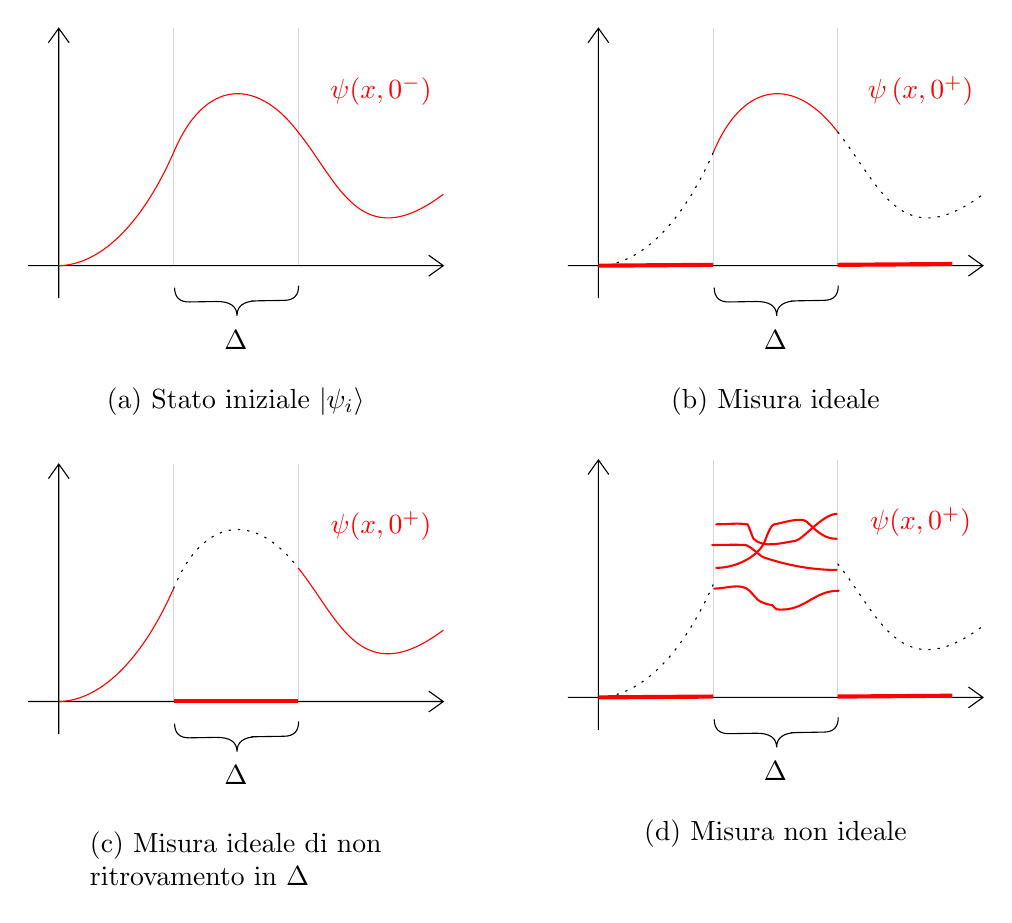
\begin{tikzpicture}[x=0.75pt,y=0.75pt,yscale=-1,xscale=1]
%uncomment if require: \path (0,528); %set diagram left start at 0, and has height of 528

%Shape: Axis 2D [id:dp8292800199787969] 
\draw  (350,184.4) -- (550,184.4)(364.71,70) -- (364.71,200) (543,179.4) -- (550,184.4) -- (543,189.4) (359.71,77) -- (364.71,70) -- (369.71,77)  ;
%Curve Lines [id:da21961617274147582] 
\draw  [dash pattern={on 0.84pt off 2.51pt}]  (364.71,184.4) .. controls (384.5,184) and (404.5,165) .. (420,130) ;


%Curve Lines [id:da6544732750416009] 
\draw [color={rgb, 255:red, 255; green, 0; blue, 0 }  ,draw opacity=1 ]   (420,130) .. controls (434.5,95) and (459.5,93) .. (480,120) ;


%Curve Lines [id:da25131822572947504] 
\draw  [dash pattern={on 0.84pt off 2.51pt}]  (480,120) .. controls (499.5,144) and (510,180) .. (550,150) ;


%Straight Lines [id:da5555264546254466] 
\draw [color={rgb, 255:red, 0; green, 0; blue, 0 }  ,draw opacity=0.16 ]   (420,70) -- (420,184) ;


%Straight Lines [id:da35060730211001423] 
\draw [color={rgb, 255:red, 255; green, 0; blue, 0 }  ,draw opacity=1 ][fill={rgb, 255:red, 54; green, 235; blue, 33 }  ,fill opacity=1 ][line width=1.5]    (364.71,184.4) -- (420,184) ;


%Straight Lines [id:da6883405875773769] 
\draw [color={rgb, 255:red, 255; green, 0; blue, 0 }  ,draw opacity=1 ][fill={rgb, 255:red, 54; green, 235; blue, 33 }  ,fill opacity=1 ][line width=1.5]    (480,184) -- (535.29,183.6) ;


%Shape: Brace [id:dp0596408730965543] 
\draw   (420.5,195) .. controls (420.58,199.67) and (422.95,201.96) .. (427.62,201.88) -- (440.49,201.67) .. controls (447.16,201.56) and (450.53,203.83) .. (450.61,208.5) .. controls (450.53,203.83) and (453.82,201.44) .. (460.49,201.33)(457.49,201.38) -- (473.37,201.12) .. controls (478.04,201.04) and (480.33,198.67) .. (480.25,194) ;
%Straight Lines [id:da6648444148915165] 
\draw [color={rgb, 255:red, 0; green, 0; blue, 0 }  ,draw opacity=0.16 ]   (480,70) -- (480,184) ;


%Shape: Axis 2D [id:dp4326237444016172] 
\draw  (90,184.4) -- (290,184.4)(104.71,70) -- (104.71,200) (283,179.4) -- (290,184.4) -- (283,189.4) (99.71,77) -- (104.71,70) -- (109.71,77)  ;
%Curve Lines [id:da0018502569924550016] 
\draw [color={rgb, 255:red, 255; green, 0; blue, 0 }  ,draw opacity=1 ]   (104.71,184.4) .. controls (124.5,184) and (144.5,165) .. (160,130) ;


%Curve Lines [id:da9006344879421362] 
\draw [color={rgb, 255:red, 255; green, 0; blue, 0 }  ,draw opacity=1 ]   (160,130) .. controls (174.5,95) and (199.5,93) .. (220,120) ;


%Curve Lines [id:da6523707803574752] 
\draw [color={rgb, 255:red, 255; green, 0; blue, 0 }  ,draw opacity=1 ]   (220,120) .. controls (239.5,144) and (250,180) .. (290,150) ;


%Straight Lines [id:da513106852520784] 
\draw [color={rgb, 255:red, 0; green, 0; blue, 0 }  ,draw opacity=0.16 ]   (160,70) -- (160,184) ;


%Shape: Brace [id:dp5621992263610398] 
\draw   (160.5,195) .. controls (160.58,199.67) and (162.95,201.96) .. (167.62,201.88) -- (180.49,201.67) .. controls (187.16,201.56) and (190.53,203.83) .. (190.61,208.5) .. controls (190.53,203.83) and (193.82,201.44) .. (200.49,201.33)(197.49,201.38) -- (213.37,201.12) .. controls (218.04,201.04) and (220.33,198.67) .. (220.25,194) ;
%Straight Lines [id:da38638140982840774] 
\draw [color={rgb, 255:red, 0; green, 0; blue, 0 }  ,draw opacity=0.16 ]   (220,70) -- (220,184) ;


%Shape: Axis 2D [id:dp49952262944411907] 
\draw  (350,392.4) -- (550,392.4)(364.71,278) -- (364.71,408) (543,387.4) -- (550,392.4) -- (543,397.4) (359.71,285) -- (364.71,278) -- (369.71,285)  ;
%Curve Lines [id:da9955621212244545] 
\draw  [dash pattern={on 0.84pt off 2.51pt}]  (364.71,392.4) .. controls (384.5,392) and (404.5,373) .. (420,338) ;


%Curve Lines [id:da597211341967508] 
\draw  [dash pattern={on 0.84pt off 2.51pt}]  (480,328) .. controls (499.5,352) and (510,388) .. (550,358) ;


%Straight Lines [id:da7612949723055946] 
\draw [color={rgb, 255:red, 0; green, 0; blue, 0 }  ,draw opacity=0.16 ]   (420,278) -- (420,392) ;


%Straight Lines [id:da8958203480784113] 
\draw [color={rgb, 255:red, 255; green, 0; blue, 0 }  ,draw opacity=1 ][fill={rgb, 255:red, 54; green, 235; blue, 33 }  ,fill opacity=1 ][line width=1.5]    (364.71,392.4) -- (420,392) ;


%Straight Lines [id:da17219676480712076] 
\draw [color={rgb, 255:red, 255; green, 0; blue, 0 }  ,draw opacity=1 ][fill={rgb, 255:red, 54; green, 235; blue, 33 }  ,fill opacity=1 ][line width=1.5]    (480,392) -- (535.29,391.6) ;


%Shape: Brace [id:dp006778926571109789] 
\draw   (420.5,403) .. controls (420.58,407.67) and (422.95,409.96) .. (427.62,409.88) -- (440.49,409.67) .. controls (447.16,409.56) and (450.53,411.83) .. (450.61,416.5) .. controls (450.53,411.83) and (453.82,409.44) .. (460.49,409.33)(457.49,409.38) -- (473.37,409.12) .. controls (478.04,409.04) and (480.33,406.67) .. (480.25,402) ;
%Straight Lines [id:da8894990152362152] 
\draw [color={rgb, 255:red, 0; green, 0; blue, 0 }  ,draw opacity=0.16 ]   (480,278) -- (480,392) ;


%Shape: Free Drawing [id:dp45303562420740495] 
\draw  [color={rgb, 255:red, 255; green, 0; blue, 0 }  ,draw opacity=1 ][line width=0.75] [line join = round][line cap = round] (421.5,309) .. controls (426.5,309) and (431.54,308.34) .. (436.5,309) .. controls (436.92,309.06) and (439.02,315.52) .. (439.5,316) .. controls (444.22,320.72) and (452.89,317.94) .. (459.5,317) .. controls (463.2,316.47) and (472.79,304) .. (479.5,304) ;
%Shape: Free Drawing [id:dp11301025054340808] 
\draw  [color={rgb, 255:red, 255; green, 0; blue, 0 }  ,draw opacity=1 ][line width=0.75] [line join = round][line cap = round] (421.5,330) .. controls (430.7,330) and (441.03,324.95) .. (444.5,318) .. controls (445.46,316.09) and (447.38,309.35) .. (449.5,309) .. controls (453.64,308.31) and (459.53,306.21) .. (463.5,307) .. controls (466.58,307.62) and (470.73,316) .. (479.5,316) ;
%Shape: Free Drawing [id:dp1219300915173025] 
\draw  [color={rgb, 255:red, 255; green, 0; blue, 0 }  ,draw opacity=1 ][line width=0.75] [line join = round][line cap = round] (420.5,340) .. controls (426.18,340) and (433.49,336.99) .. (437.5,341) .. controls (441.64,345.14) and (440.82,346.46) .. (448.5,348) .. controls (449.42,348.18) and (449.56,349.91) .. (450.5,350) .. controls (464.41,351.26) and (467.83,341) .. (480.5,341) ;
%Shape: Free Drawing [id:dp6499401343401028] 
\draw  [color={rgb, 255:red, 255; green, 0; blue, 0 }  ,draw opacity=1 ][line width=0.75] [line join = round][line cap = round] (419.5,319) .. controls (424.83,319) and (430.18,318.67) .. (435.5,319) .. controls (437.63,319.13) and (442.56,324.35) .. (444.5,325) .. controls (455.45,328.65) and (467.38,331) .. (479.5,331) ;
%Shape: Axis 2D [id:dp23546476358509705] 
\draw  (90,394.4) -- (290,394.4)(104.71,280) -- (104.71,410) (283,389.4) -- (290,394.4) -- (283,399.4) (99.71,287) -- (104.71,280) -- (109.71,287)  ;
%Curve Lines [id:da6199691430940644] 
\draw [color={rgb, 255:red, 255; green, 0; blue, 0 }  ,draw opacity=1 ]   (104.71,394.4) .. controls (124.5,394) and (144.5,375) .. (160,340) ;


%Curve Lines [id:da1207198200128774] 
\draw [color={rgb, 255:red, 0; green, 0; blue, 0 }  ,draw opacity=1 ] [dash pattern={on 0.84pt off 2.51pt}]  (160,340) .. controls (174.5,305) and (199.5,303) .. (220,330) ;


%Curve Lines [id:da3558938944118475] 
\draw [color={rgb, 255:red, 255; green, 0; blue, 0 }  ,draw opacity=1 ]   (220,330) .. controls (239.5,354) and (250,390) .. (290,360) ;


%Straight Lines [id:da3017560485704682] 
\draw [color={rgb, 255:red, 0; green, 0; blue, 0 }  ,draw opacity=0.16 ]   (160,280) -- (160,394) ;


%Straight Lines [id:da11067727122637927] 
\draw [color={rgb, 255:red, 255; green, 0; blue, 0 }  ,draw opacity=1 ][fill={rgb, 255:red, 54; green, 235; blue, 33 }  ,fill opacity=1 ][line width=1.5]    (160,394) -- (220,394) ;


%Shape: Brace [id:dp4532126138378527] 
\draw   (160.5,405) .. controls (160.58,409.67) and (162.95,411.96) .. (167.62,411.88) -- (180.49,411.67) .. controls (187.16,411.56) and (190.53,413.83) .. (190.61,418.5) .. controls (190.53,413.83) and (193.82,411.44) .. (200.49,411.33)(197.49,411.38) -- (213.37,411.12) .. controls (218.04,411.04) and (220.33,408.67) .. (220.25,404) ;
%Straight Lines [id:da5980711218008583] 
\draw [color={rgb, 255:red, 0; green, 0; blue, 0 }  ,draw opacity=0.16 ]   (220,280) -- (220,394) ;



% Text Node
\draw (450,220) node [color={rgb, 255:red, 0; green, 0; blue, 0 }  ,opacity=1 ]  {$\Delta $};
% Text Node
\draw (520,100) node   {$\textcolor[rgb]{1,0,0}{\psi \left( x,0^{+}\right)}$};
% Text Node
\draw (190,220) node [color={rgb, 255:red, 0; green, 0; blue, 0 }  ,opacity=1 ]  {$\Delta $};
% Text Node
\draw (260,100) node   {$\textcolor[rgb]{1,0,0}{\psi(x,0^{-})}$};
% Text Node
\draw (190,250) node  [align=left] {(a) Stato iniziale $\displaystyle |\psi _{i} \rangle $};
% Text Node
\draw (450,250) node  [align=left] {(b) Misura ideale};
% Text Node
\draw (450,428) node [color={rgb, 255:red, 0; green, 0; blue, 0 }  ,opacity=1 ]  {$\Delta $};
% Text Node
\draw (520,308) node   {$\textcolor[rgb]{1,0,0}{\psi(x,0^{+})}$};
% Text Node
\draw (190,470) node  [align=left] {(c) Misura ideale di non\\ritrovamento in $\displaystyle \Delta $};
% Text Node
\draw (450,458) node  [align=left] {(d) Misura non ideale};
% Text Node
\draw (190,430) node [color={rgb, 255:red, 0; green, 0; blue, 0 }  ,opacity=1 ]  {$\Delta $};
% Text Node
\draw (260,310) node   {$\textcolor[rgb]{1,0,0}{\psi(x,0^{+})}$};


\end{tikzpicture}
\caption{Differenti risultati di una misura.}
\label{fig:mqmeasures}
\end{center}
\end{figure}

A $t=0$ viene eseguita una misura (di prima specie) di posizione, e la particella viene trovata nell'intervallo $\Delta \subset \bb{R}$.\\
Poiché tutte le misure di posizione seguenti dovranno dare lo stesso risultato, $\braket{x|\psi_i(0^+)}$ è nulla su tutto $\bb{R}$, tranne che in $\Delta$: sappiamo con certezza che la particella deve trovarsi in $\Delta$.\\
Se la misura non è stata ideale non sappiamo nient'altro: i valori assunti in $\Delta$ potrebbero essere \textit{qualsiasi}. Se invece la misura è stata ideale sappiamo di non aver \q{deturpato eccessivamente} la situazione originaria, e perciò la nuova funzione d'onda in $\Delta$ ha lo stesso andamento che aveva prima della misura, come rappresentato in figura \ref{fig:mqmeasures}b e \ref{fig:mqmeasures}d.\\
Cosa sarebbe successo se invece la misura \textbf{non} avesse trovato la particella in $\Delta$?\\
Anche in questo caso, lo stato del sistema sarebbe cambiato drasticamente. Anche facendo una misura ideale, infatti, la nuova situazione è quella illustrata in figura \ref{fig:mqmeasures}c.\\
Classicamente ciò è assurdo: non avendo trovato la particella, effettivamente non vi è stata alcuna \textit{interazione} tra rivelatore e particella, e quindi ci aspettiamo di non aver modificato nulla.\\
In \MQ, invece, basta semplicemente \textit{avere un'informazione in più} - che ci sia o non ci sia una particella in un certo range - per modificare l'intera funzione d'onda.\\
Questa è parte della caratteristica non località della \MQ: a distanze arbitrariamente grandi la funzione d'onda risente di una misura fatta in un dato range!
\end{document}

